\documentclass[25pt, a0paper, portrait, blockverticalspace=.5cm]{tikzposter}
\usepackage[utf8]{inputenc}
\usepackage{amssymb,amsfonts,amsmath,mathtext,mathtools}
\usepackage{xfrac}
\usepackage{enumitem}


\let\vec\oldvec
\newcommand{\vec}[1]{\boldsymbol{#1}}


\title{
	\parbox{\linewidth}{\centering
		Magneto-Optical Structure of the NICA Collider with High Critical Energy\
	}
}
\author{S.D. KOLOKOLCHIKOV\textsuperscript{1}, Y.V. SENICHEV\textsuperscript{1}, E.M. SYRESIN\textsuperscript{2}}
\institute{
	\textsuperscript{1} Institute for Nuclear Research of the Russian Academy of Sciences, Moscow, Russia\\
	\textsuperscript{2} Joint Institute for Nuclear Researches, Dubna, Russia
}

\usetheme{Simple}
\usecolorstyle{Russia}
\colorlet{blocktitlefgcolor}{black}

\usepackage{caption}
\captionsetup{font=large}
\usepackage{multicol}
\setlength\columnsep{1.5cm}

\begin{document}

\maketitle

\begin{columns}
	\column{.5}
	\block{INTRODUCTION}{
		\par For proton option of NICA collider, it is necessary to cross the transition energy ($\gamma_{tr}=7,1$). For this reason, a magneto-optical structure with a high critical energy ($\gamma_{tr}=15$) is considered. In this case, methods of increasing the critical energy for the proton option of the NICA collider are investigated. The method of superperiodic modulation of quadrupole gradients is applied. The selection of sextupoles is carried out to suppress the natural chromaticity and compensate for the sextupole component. The Twiss parameters for the proposed structures are given, as well as the dynamic apertures and working points are investigated.\\ 
		\par An important requirement in the design of a magneto-optical structure is to ensure zero dispersion in straight sections to ensure the movement of particles along the equilibrium orbit in these sections. This requirement is easily implemented in the case of creating regular arcs composed of identical superperiods. However, the peculiarity of the given structure of the NICA collider, the presence of missing magnets on the two extreme cells does not make it possible to create a completely regular arc of 4 identical superperiods. Thus, it is necessary to ensure the suppression of dispersion at the edges of the arc.
	}
	\column{.5}
	\block{SUPERPERIOD}{
		
	
		\begin{minipage}[t]{1.\linewidth}
			\begin{tikzpicture}
				\node (normal) at (0,0) {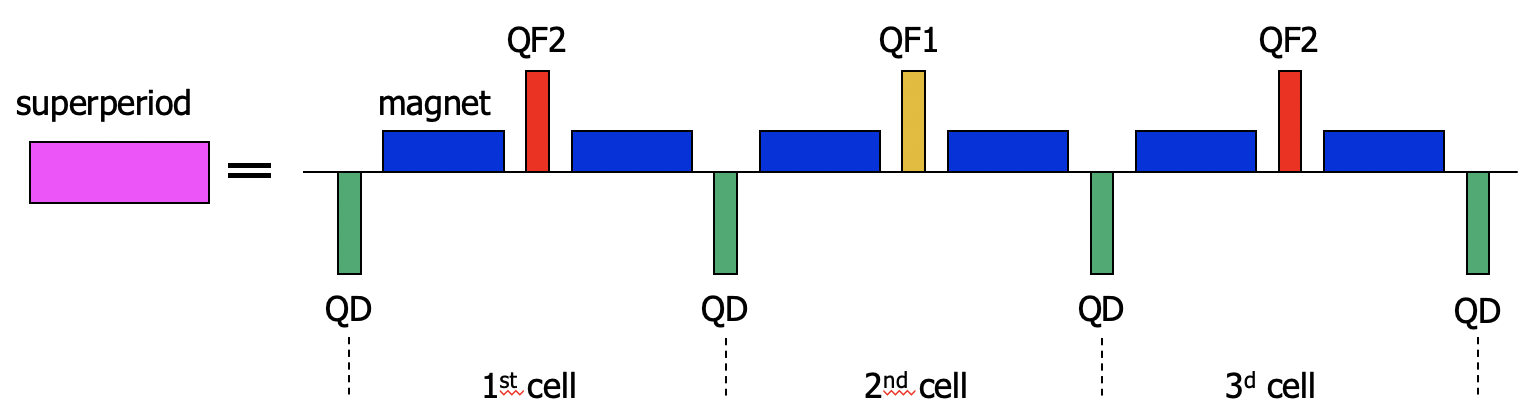
\includegraphics[width=\linewidth]{img/Superperiod}};
			\end{tikzpicture}
		\end{minipage}~~
		
		\par In the NICA structure, the regular arrangement of dipole magnets eliminates the possibility of modulating the curvature of the orbit. Therefore, to change transition energy use only the modulation of dispersion function by modulating the strength of quadrupole lenses over the superperiod. For one superperiod, the MCF is determined[1]:

		$$\alpha_{s}=\frac{1}{\nu_{x, \mathrm{arc}}^{2}}\left\{1+\frac{1}{4}\left(\frac{\bar{R}_{arc}}{\nu_{x, \text{arc}}}\right)^{4} \sum_{k=-\infty}^{\infty} \frac{g_{k}^{2}}{\left(1-k S / \nu_{x, \mathrm{arc}}\right)\left[1-\left(1-k S / \nu_{x, \mathrm{arc}}\right)^{2}\right]^{2}} \ldots\right\}$$
	}
\end{columns}

\begin{columns}
	\column{.33}
	\block{EDGE CELL SUPPRESSION}{
	
		\begin{minipage}{1\linewidth}
			\begin{tikzpicture}
			\node (cone) at (0,0) {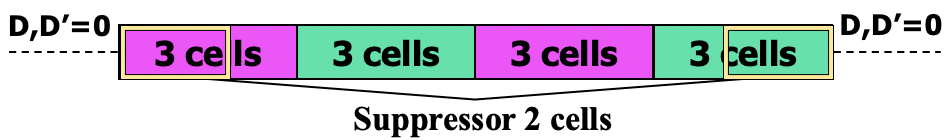
\includegraphics[width=\linewidth]{img/DS_Edge_cell}};
			\end{tikzpicture}
		\end{minipage}
		\par The edge superperiod has a missing magnet in 2 cells, thus making the collider arcs not regular and there is a need to suppress the dispersion in straight sections using the 2 additional families of QFE1 and QFE2 quadrupoles on the edge of the arc.
		\par The tune shift on the arc is equal to $\nu_{x\ arc}=3$, $\nu_{y\ arc}=3$. In the described case there is peaks of $\beta$-function on arc at quadrupoles QF2.	
	}	
	\column{.33}
	\block{2 FAMILIES SUPPRESSION }{
	
		\begin{minipage}{1\linewidth}
			\begin{tikzpicture}
			\node (cone) at (0,0) {\includegraphics[width=\linewidth]{img/DS_2_families}};
			\end{tikzpicture}
		\end{minipage}
		\par This case differs from the first, all the quadrupoles of the arc belong to the first or second family, and the suppression of dispersion is also provided by only 2 families. But to achieve the required critical energy value, it is necessary to provide a greater modulation of the quadrupole gradients than in the case of dispersion suppression by edge superperiods. In this case the phase shift on the arc becomes equal to $\nu_{x\ arc}=2,72$, $\nu_{y\ arc}=3$.
		\par The sextupoles do not compensate each other exactly.
	}
	\column{.33}
	\block{HEAVY ION MODE}{
	
		\begin{minipage}{1\linewidth}
			\begin{tikzpicture}
			\node (cone) at (0,0) {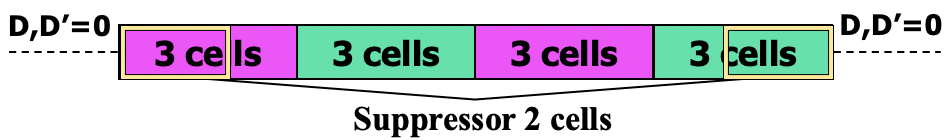
\includegraphics[width=\linewidth]{img/DS_Edge_cell}};
			\end{tikzpicture}
		\end{minipage}
		\par Ion mode structure is regular and have 12 FODO cells and contains 2 families: focusing and defocusing. Dispersion suppressed by two edge FODO cells which have a different focusing quadrupole strength when quadrupole strength in focusing family. As structure is regular there is no problems with sextupole correction. Focusing and defocusing sextupoles located near focusing and defocusing quadrupoles in the central cells.	
	}
	
\end{columns}

\begin{columns}
	\column{.33}
	\block{}{
	 
	\begin{minipage}{1\linewidth}
			\begin{tikzpicture}
			\node (cone) at (0,0) {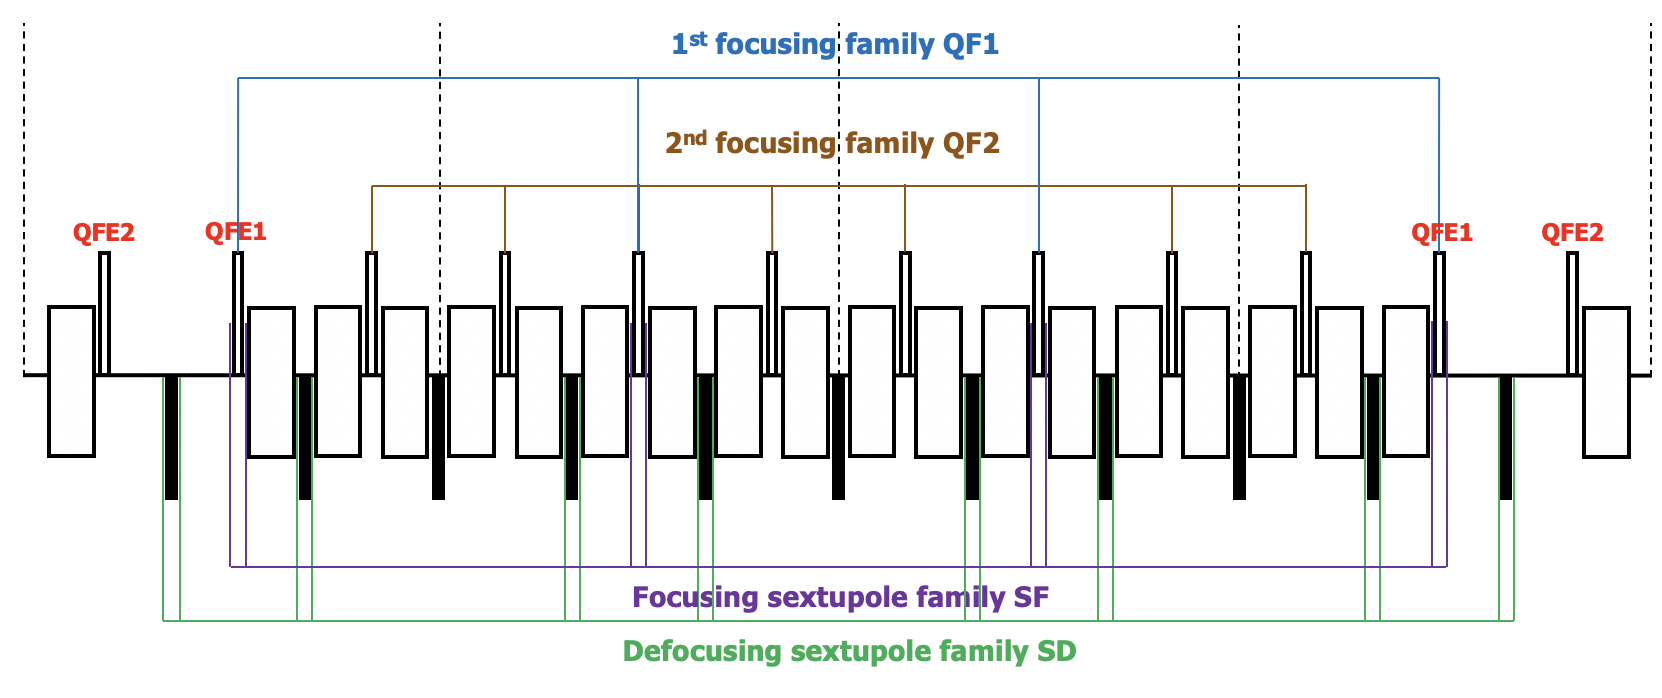
\includegraphics[width=\linewidth]{img/sextupoles_ES}};
			\end{tikzpicture}
		\end{minipage}
	}
	
	\column{.33}
	\block{}{
	 
	\begin{minipage}{1\linewidth}
			\begin{tikzpicture}
			\node (cone) at (0,0) {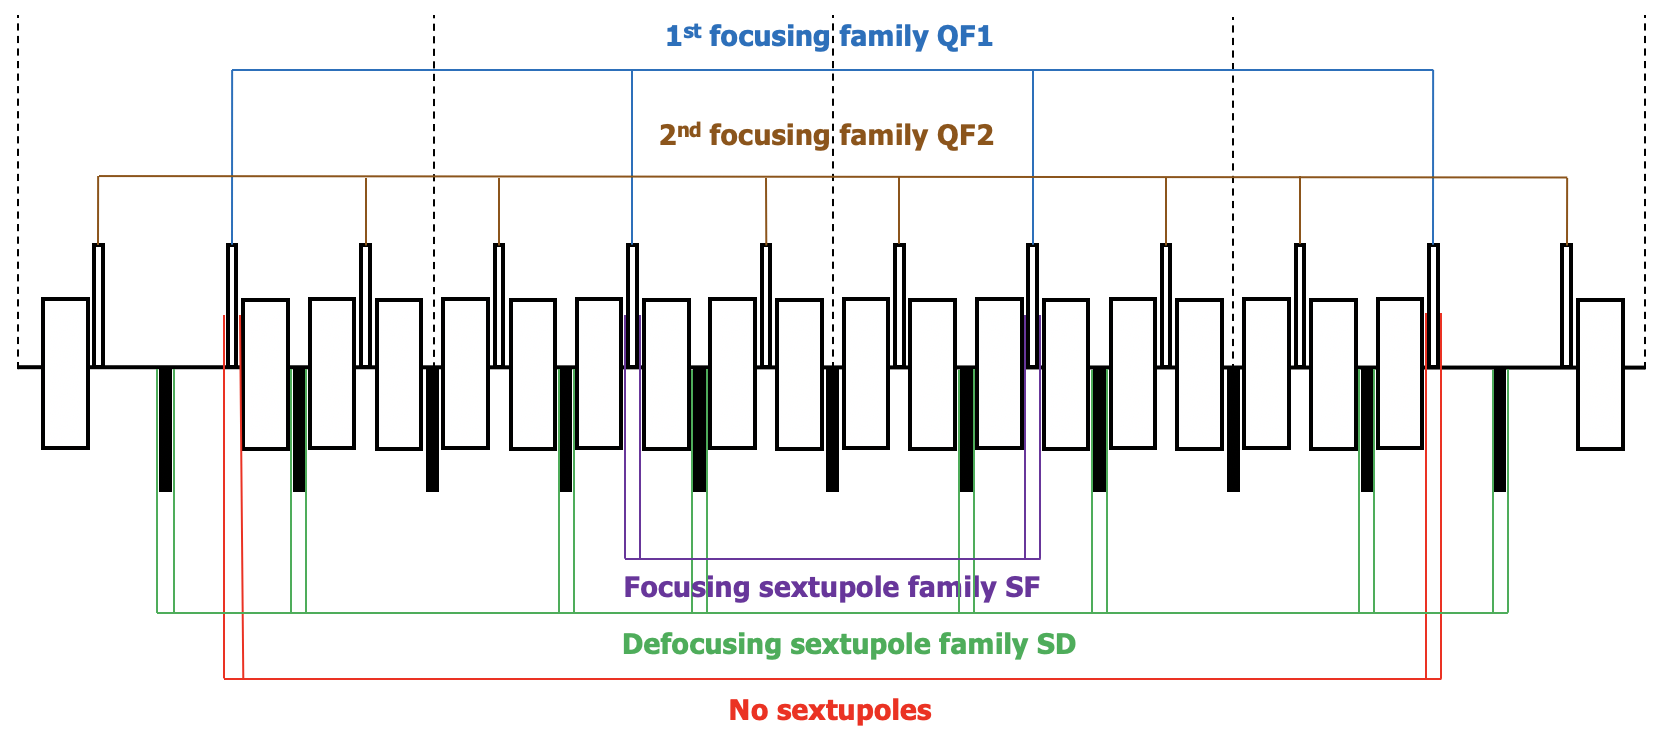
\includegraphics[width=\linewidth]{img/sextupoles_AS}};
			\end{tikzpicture}
		\end{minipage}
	}
	\column{.33}
	\block{}{
	\begin{minipage}{1\linewidth}
			\begin{tikzpicture}
			\node (cone) at (0,0) {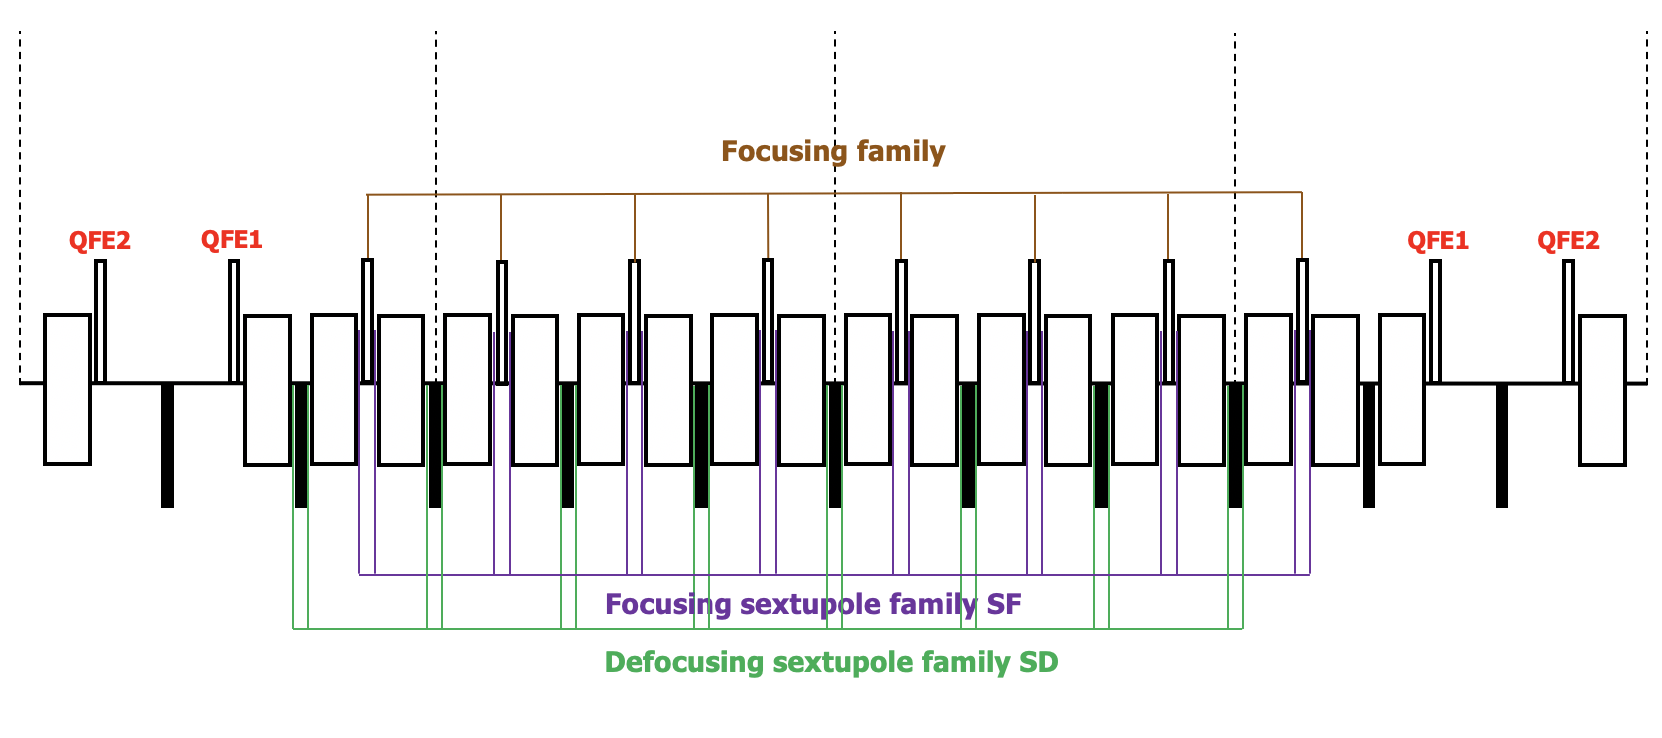
\includegraphics[width=\linewidth]{img/sextupoles_ION}};
			\end{tikzpicture}
		\end{minipage}	
	}

\end{columns}

\begin{columns}
	
	\column{.33}
	\block{}{
	\begin{minipage}{0.5\linewidth}
			\begin{tikzpicture}
			\node (cone) at (0,0) {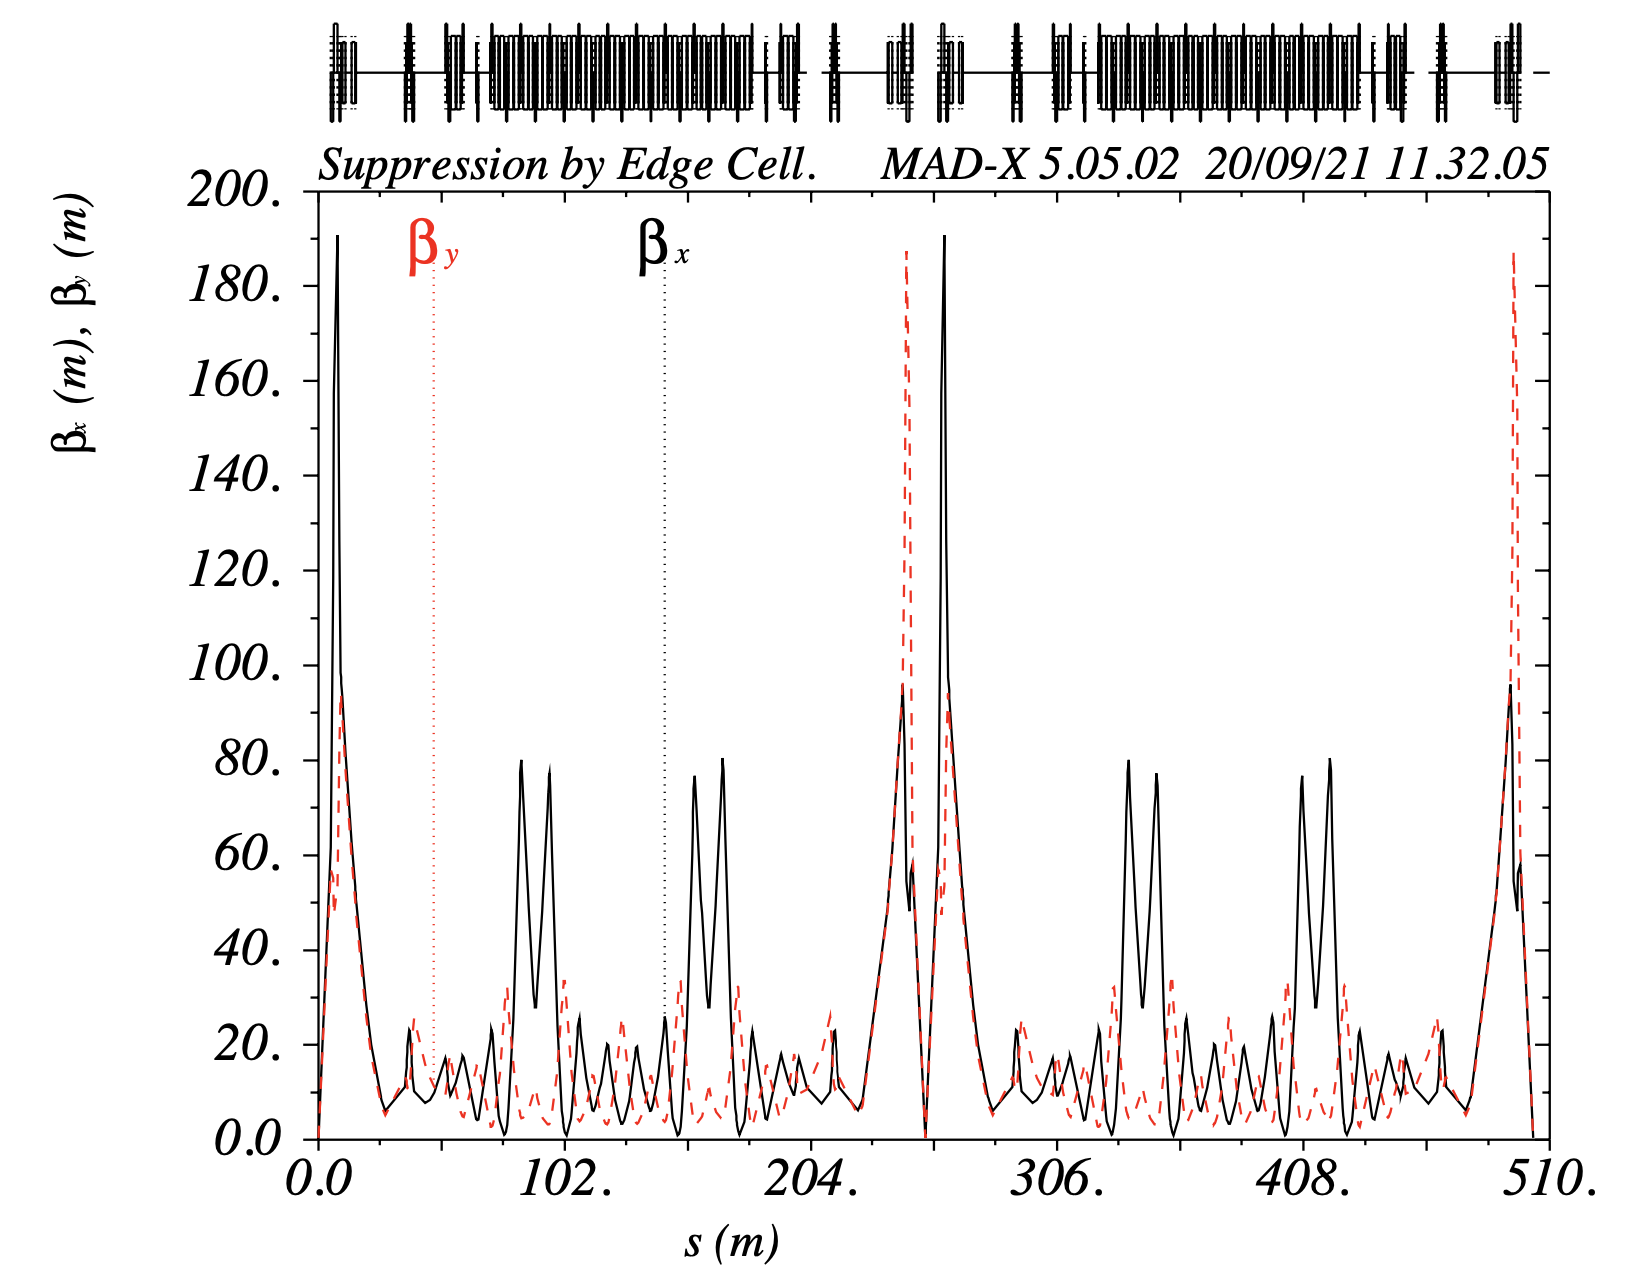
\includegraphics[width=\linewidth]{img/twiss_beta_ES}};
			\end{tikzpicture}
		\end{minipage}
		\begin{minipage}{0.5\linewidth}
			\begin{tikzpicture}
			\node (cone) at (0,0) {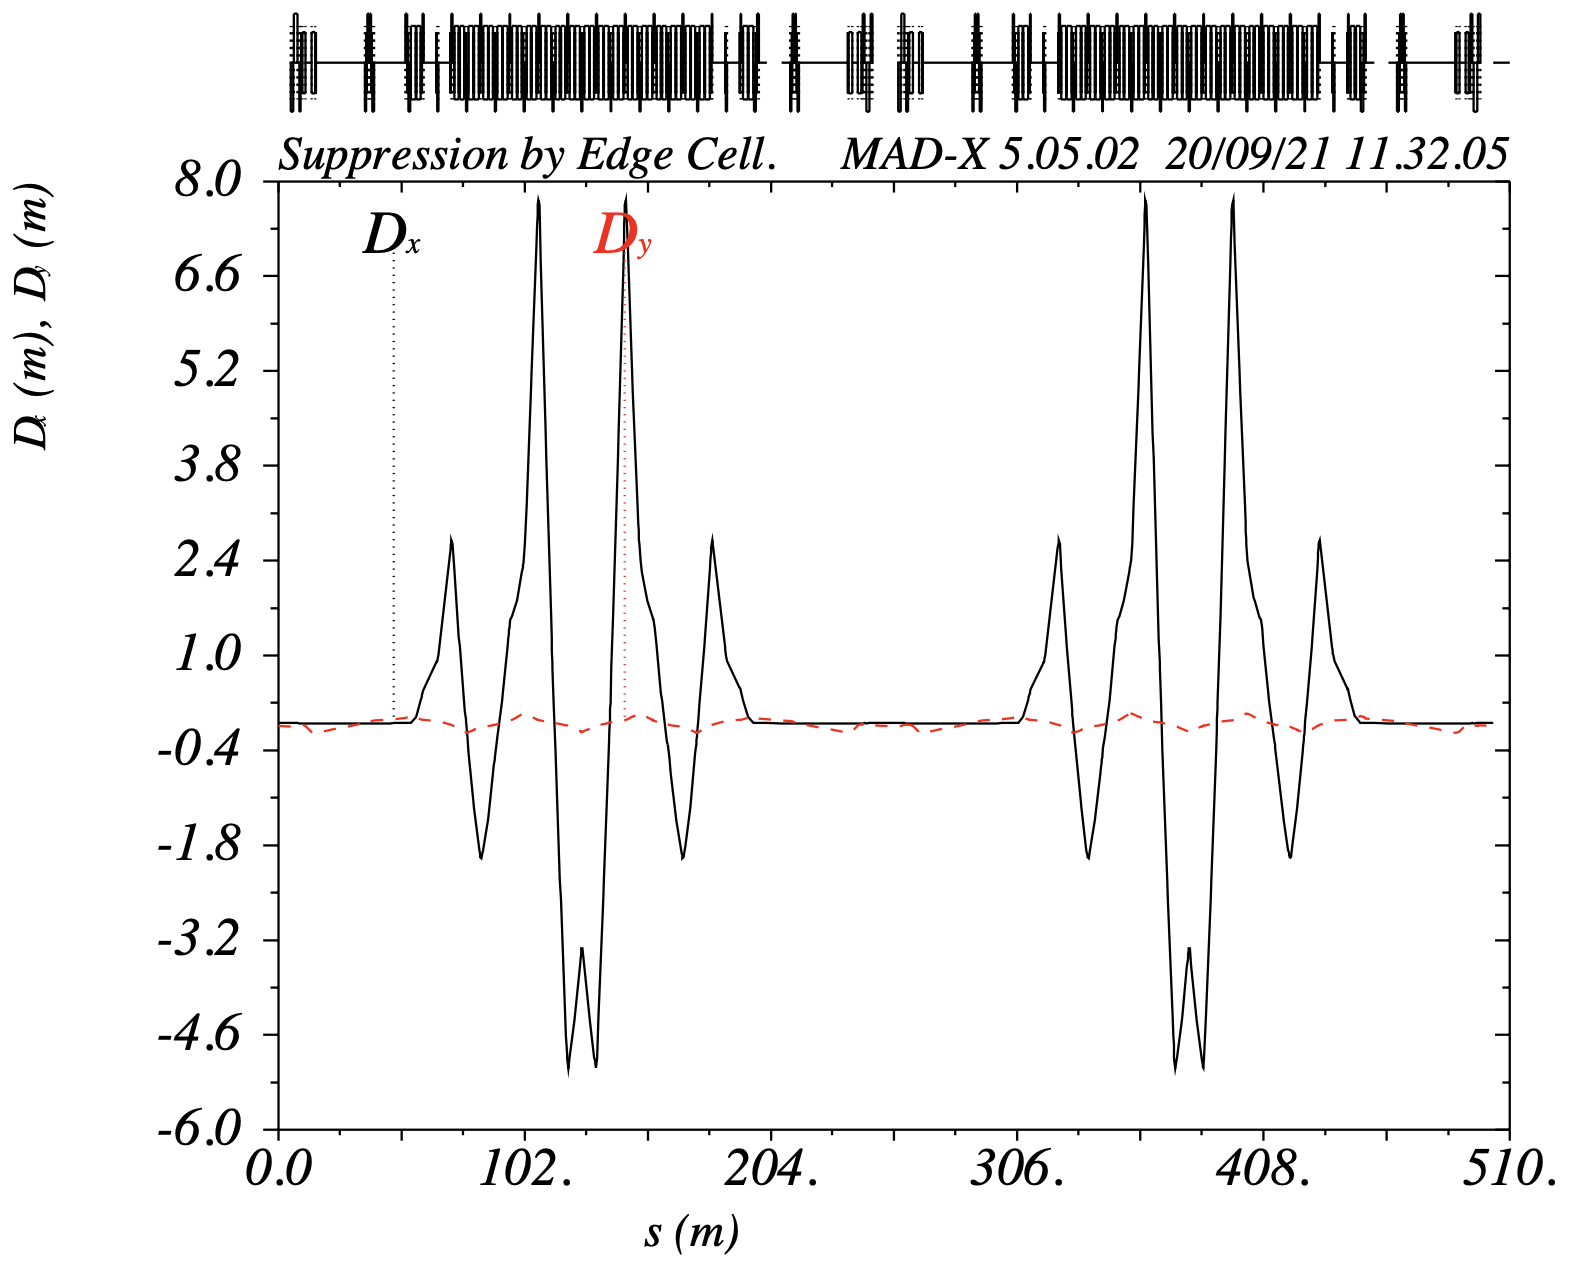
\includegraphics[width=\linewidth]{img/twiss_disp_ES}};
			\end{tikzpicture}
		\end{minipage}			
	}
		
	\column{.33}
	\block{}{
	\begin{minipage}{0.5\linewidth}
			\begin{tikzpicture}
			\node (cone) at (0,0) {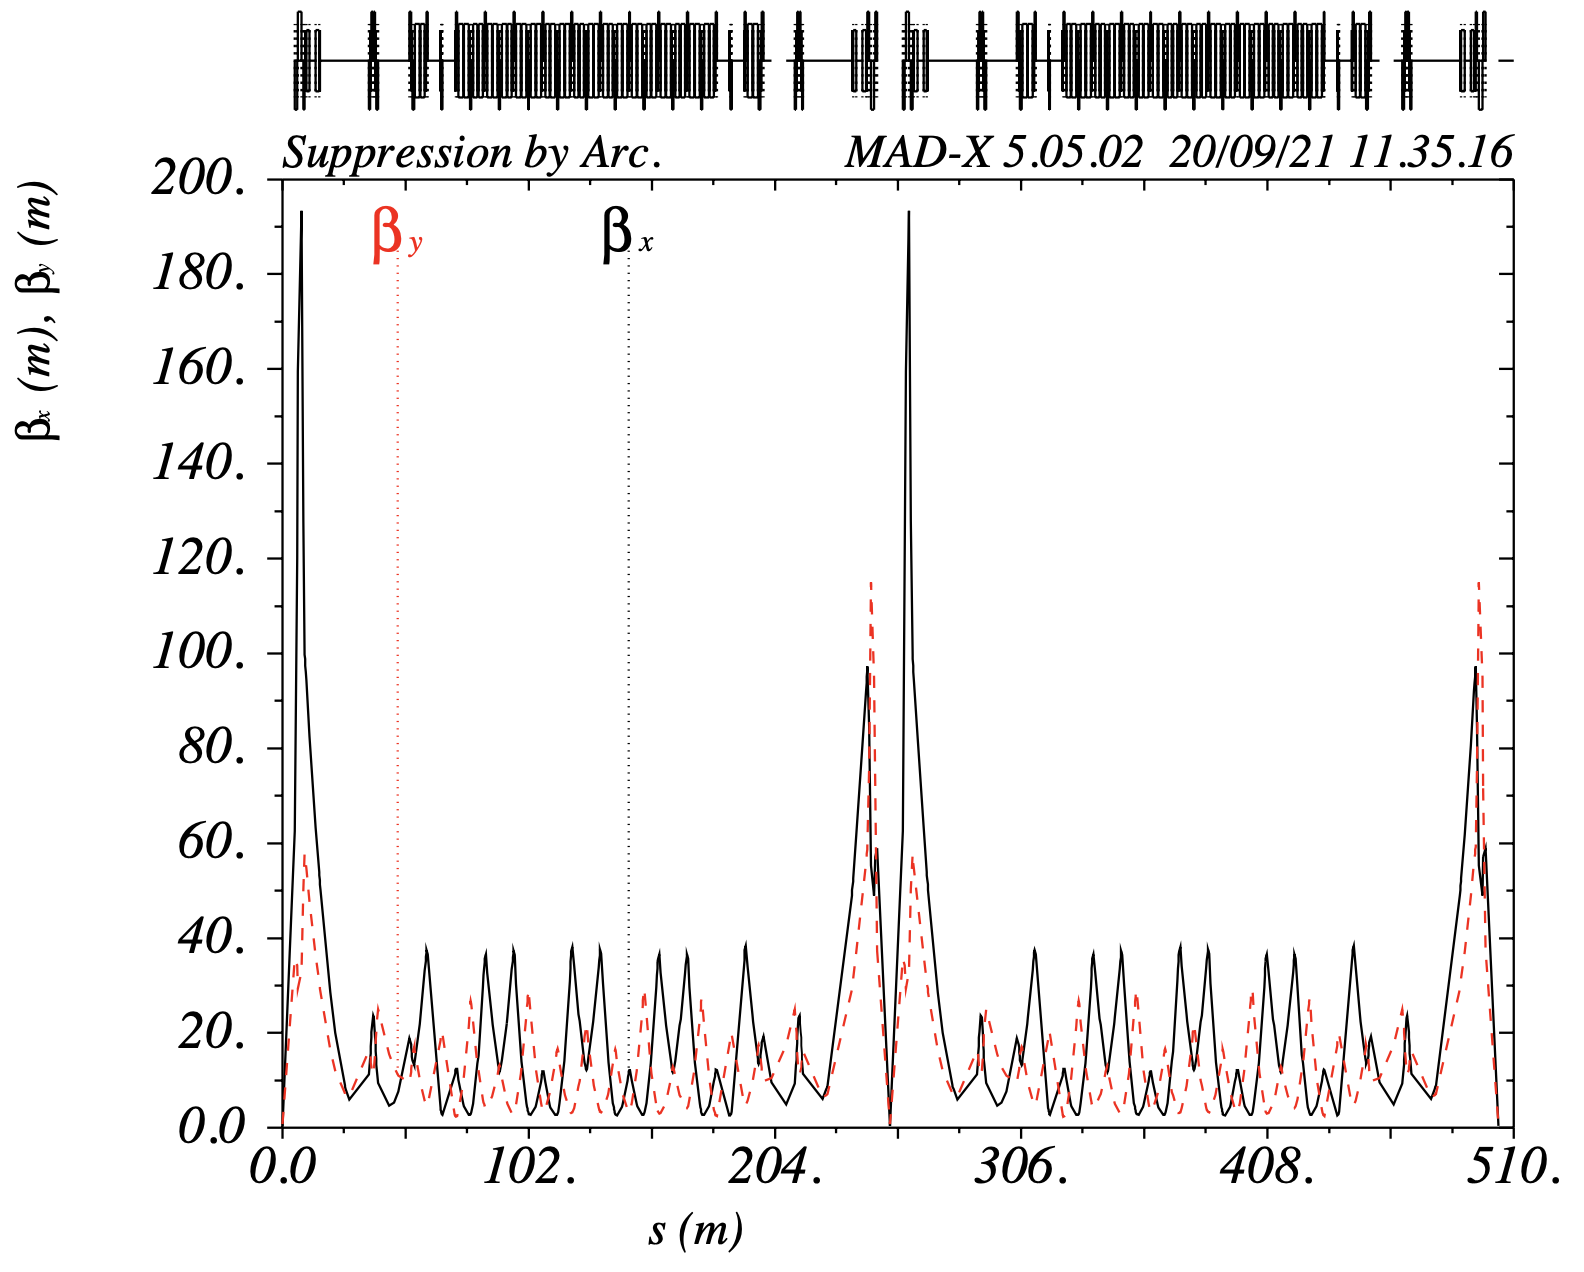
\includegraphics[width=\linewidth]{img/twiss_beta_AS}};
			\end{tikzpicture}
		\end{minipage}
		\begin{minipage}{0.5\linewidth}
			\begin{tikzpicture}
			\node (cone) at (0,0) {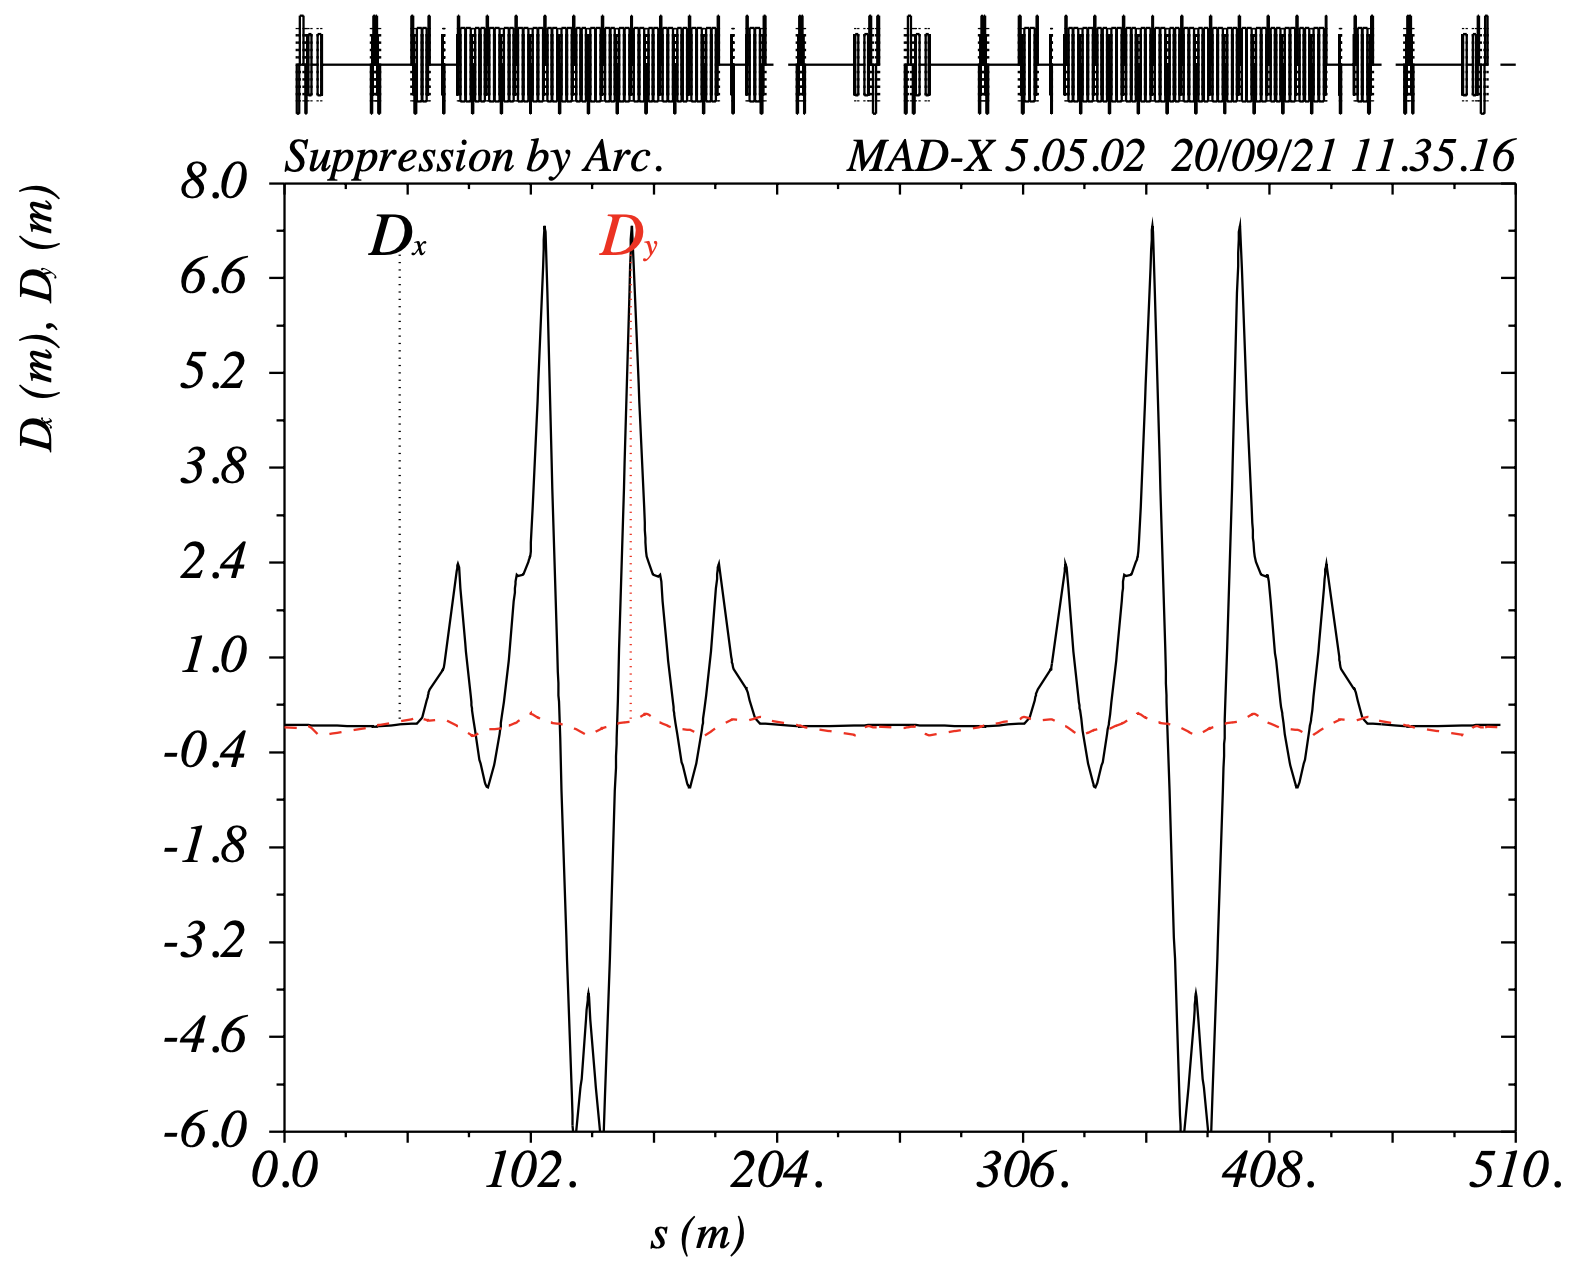
\includegraphics[width=\linewidth]{img/twiss_disp_AS}};
			\end{tikzpicture}
		\end{minipage}			
	}
	\column{.33}
	\block{}{
	\begin{minipage}{0.5\linewidth}
			\begin{tikzpicture}
			\node (cone) at (1,0) {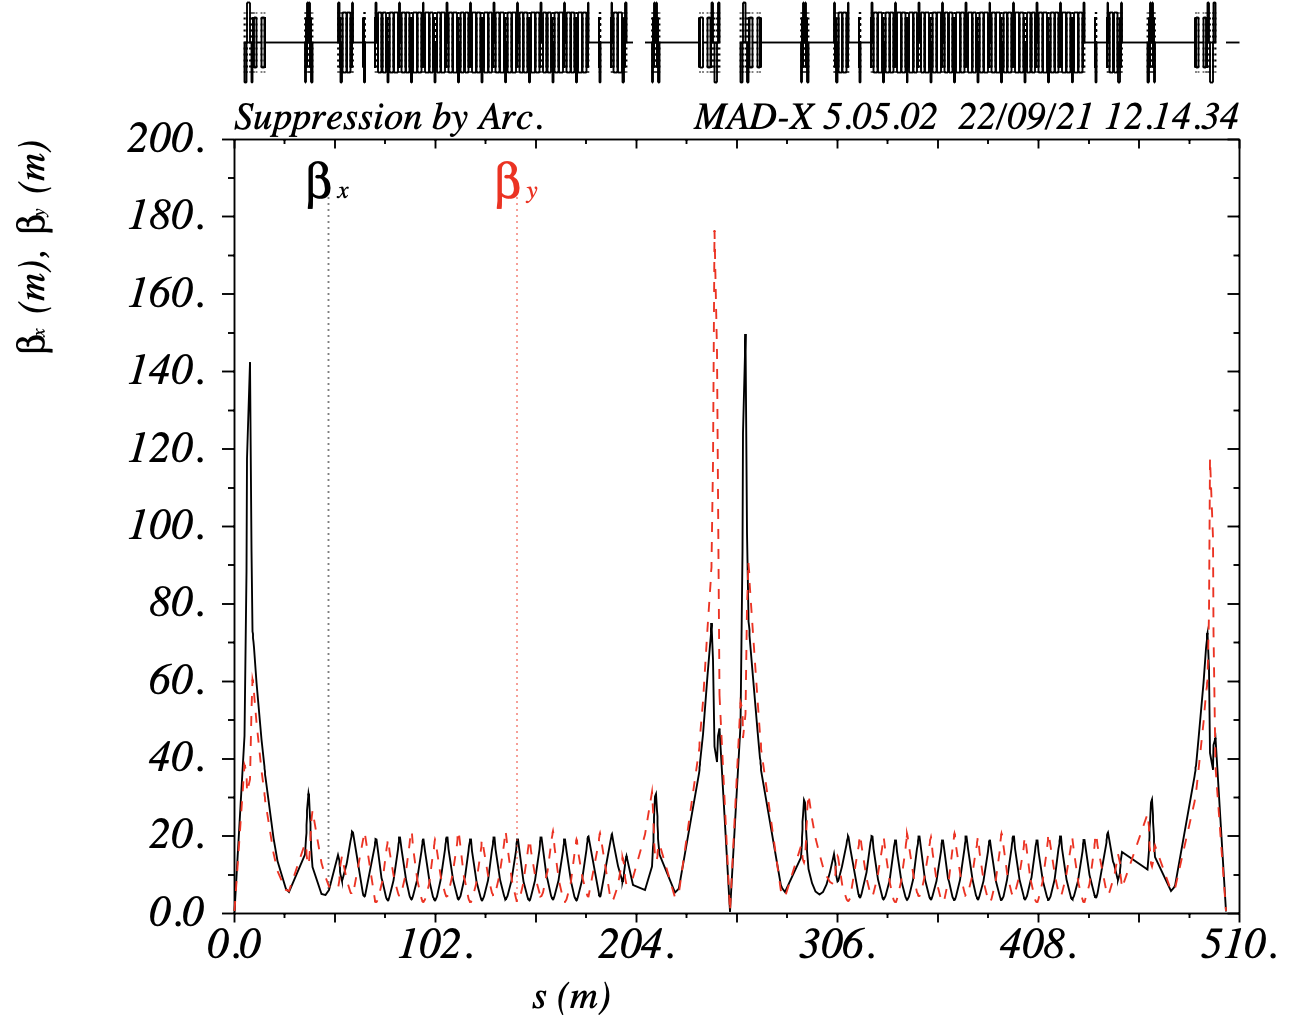
\includegraphics[width=\linewidth]{img/twiss_beta_ion}};
			\end{tikzpicture}
		\end{minipage}
		\begin{minipage}{0.5\linewidth}
			\begin{tikzpicture}
			\node (cone) at (0,0) {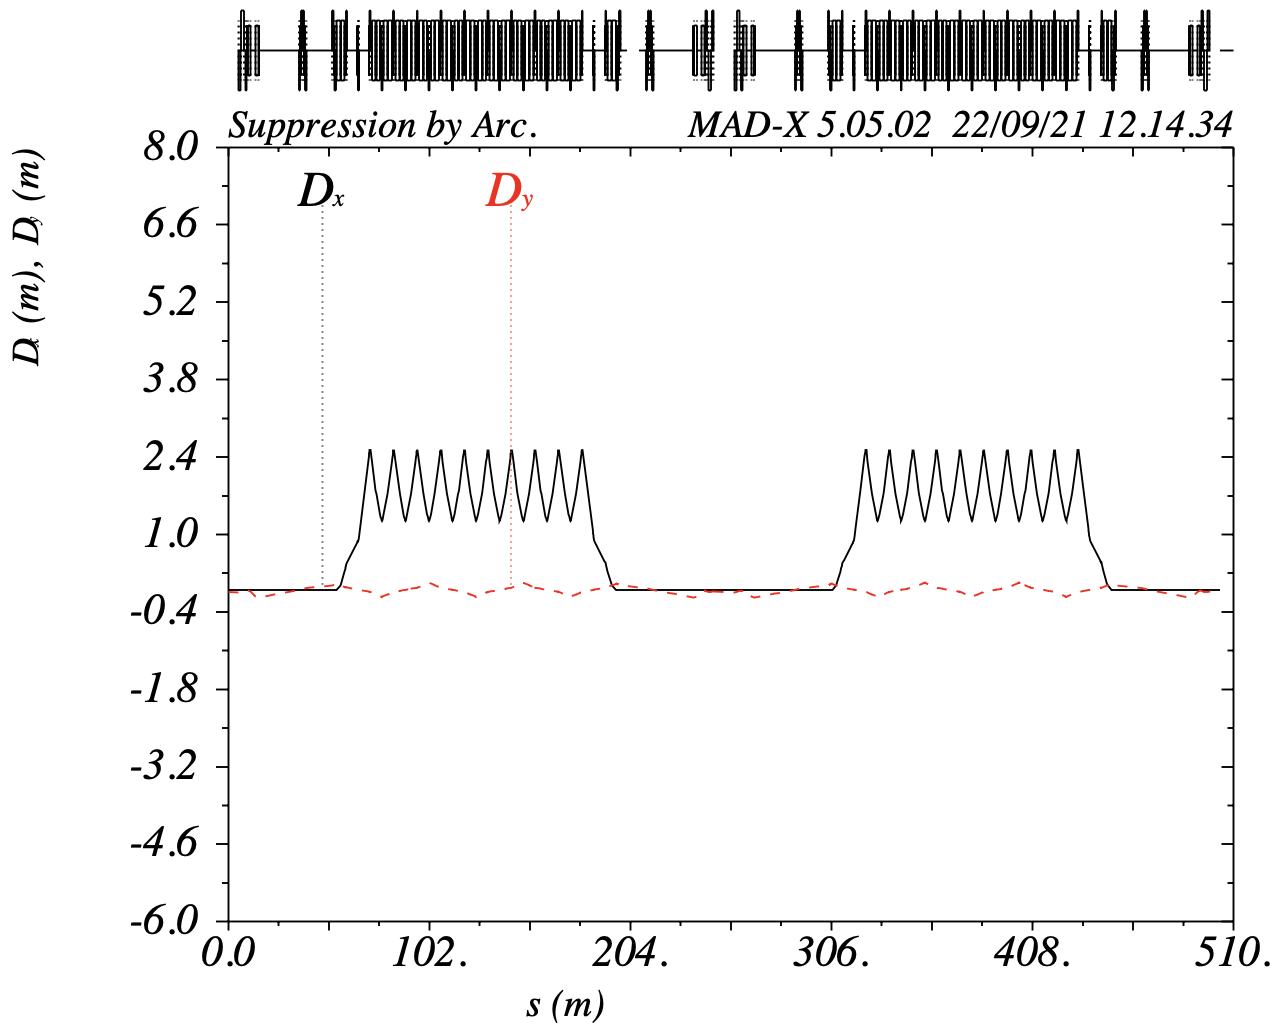
\includegraphics[width=\linewidth]{img/twiss_disp_ion}};
			\end{tikzpicture}
		\end{minipage}
	}
\end{columns}

\begin{columns}
	\column{.33}
	\block{}{
	\begin{minipage}{0.5\linewidth}
			\begin{tikzpicture}
			\node (cone) at (0,0) {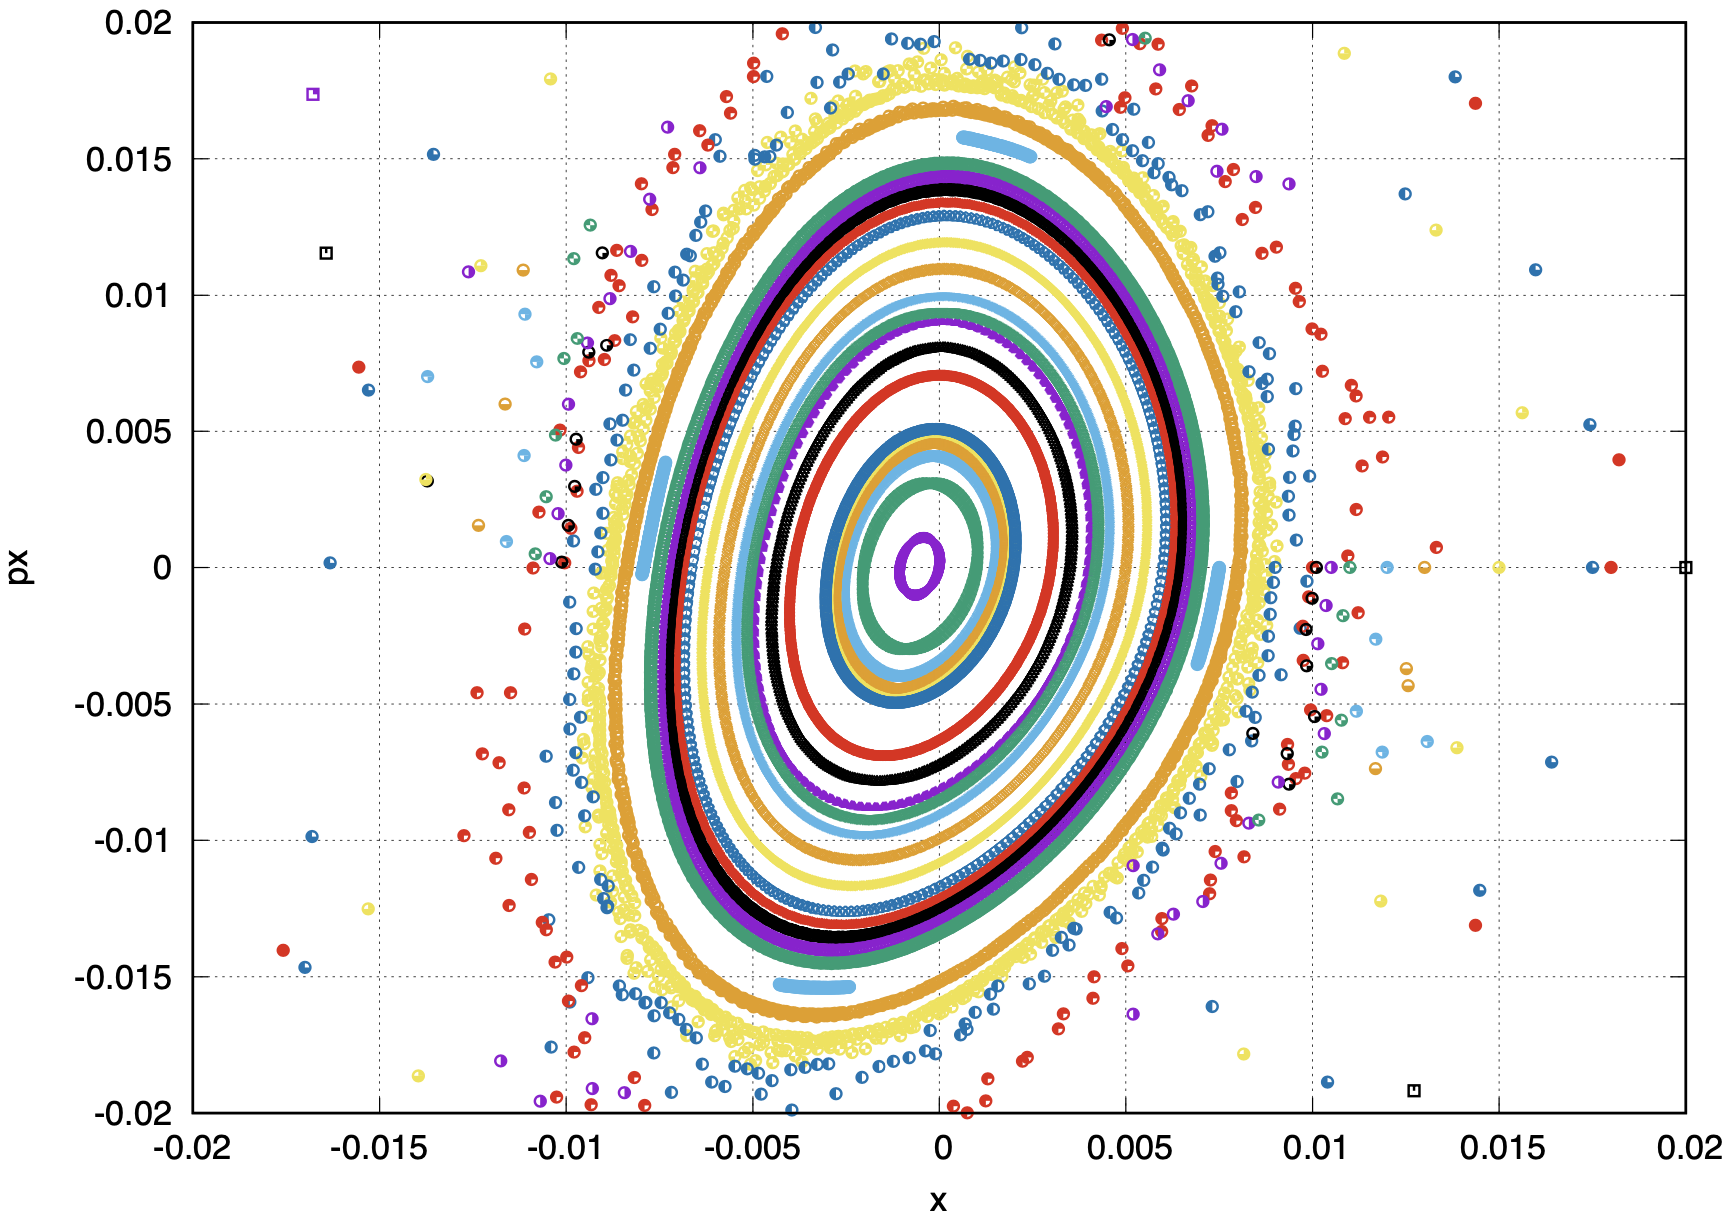
\includegraphics[width=\linewidth]{img/dyn_aper_x_ES}};
			\end{tikzpicture}
		\end{minipage}
		\begin{minipage}{0.5\linewidth}
			\begin{tikzpicture}
			\node (cone) at (0,0) {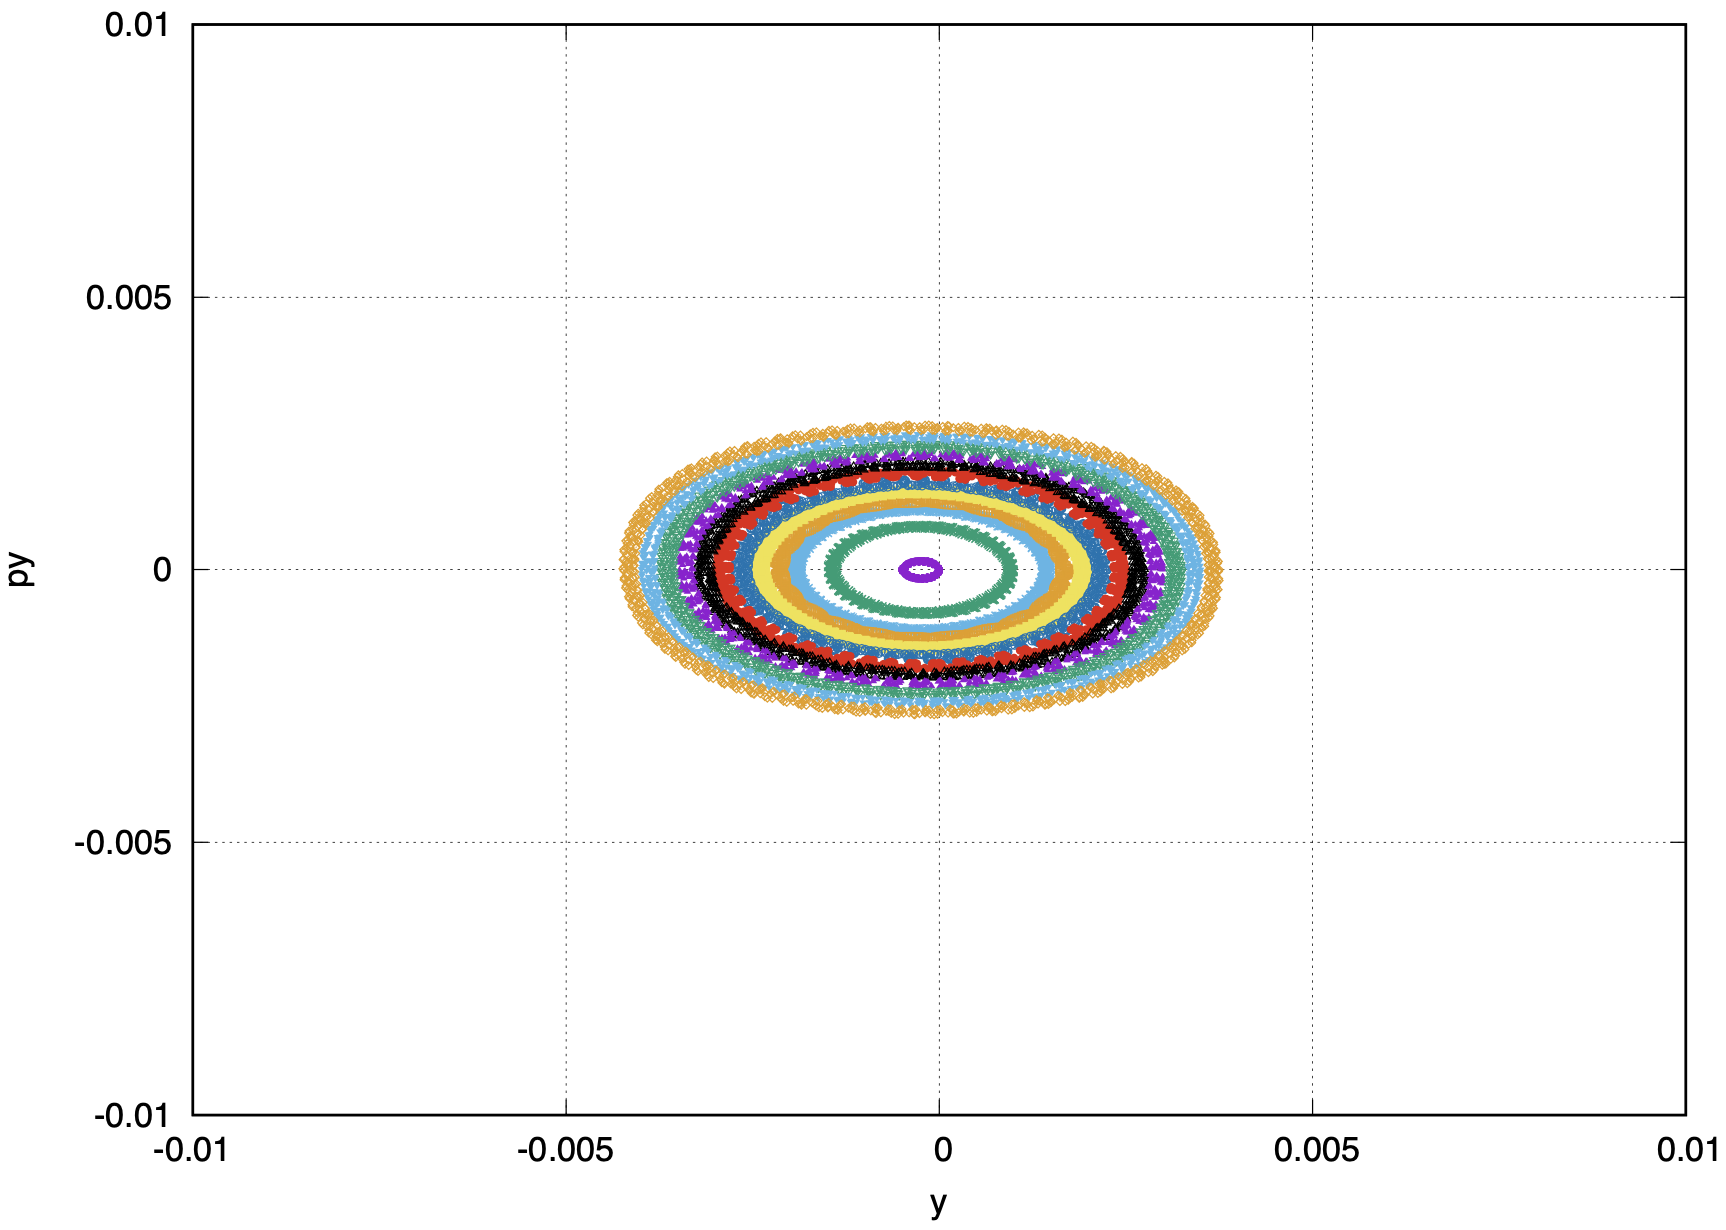
\includegraphics[width=\linewidth]{img/dyn_aper_y_ES}};
			\end{tikzpicture}
		\end{minipage}
		}
	\column{.33}
	\block{}{
	\begin{minipage}{0.5\linewidth}
			\begin{tikzpicture}
			\node (cone) at (0,0) {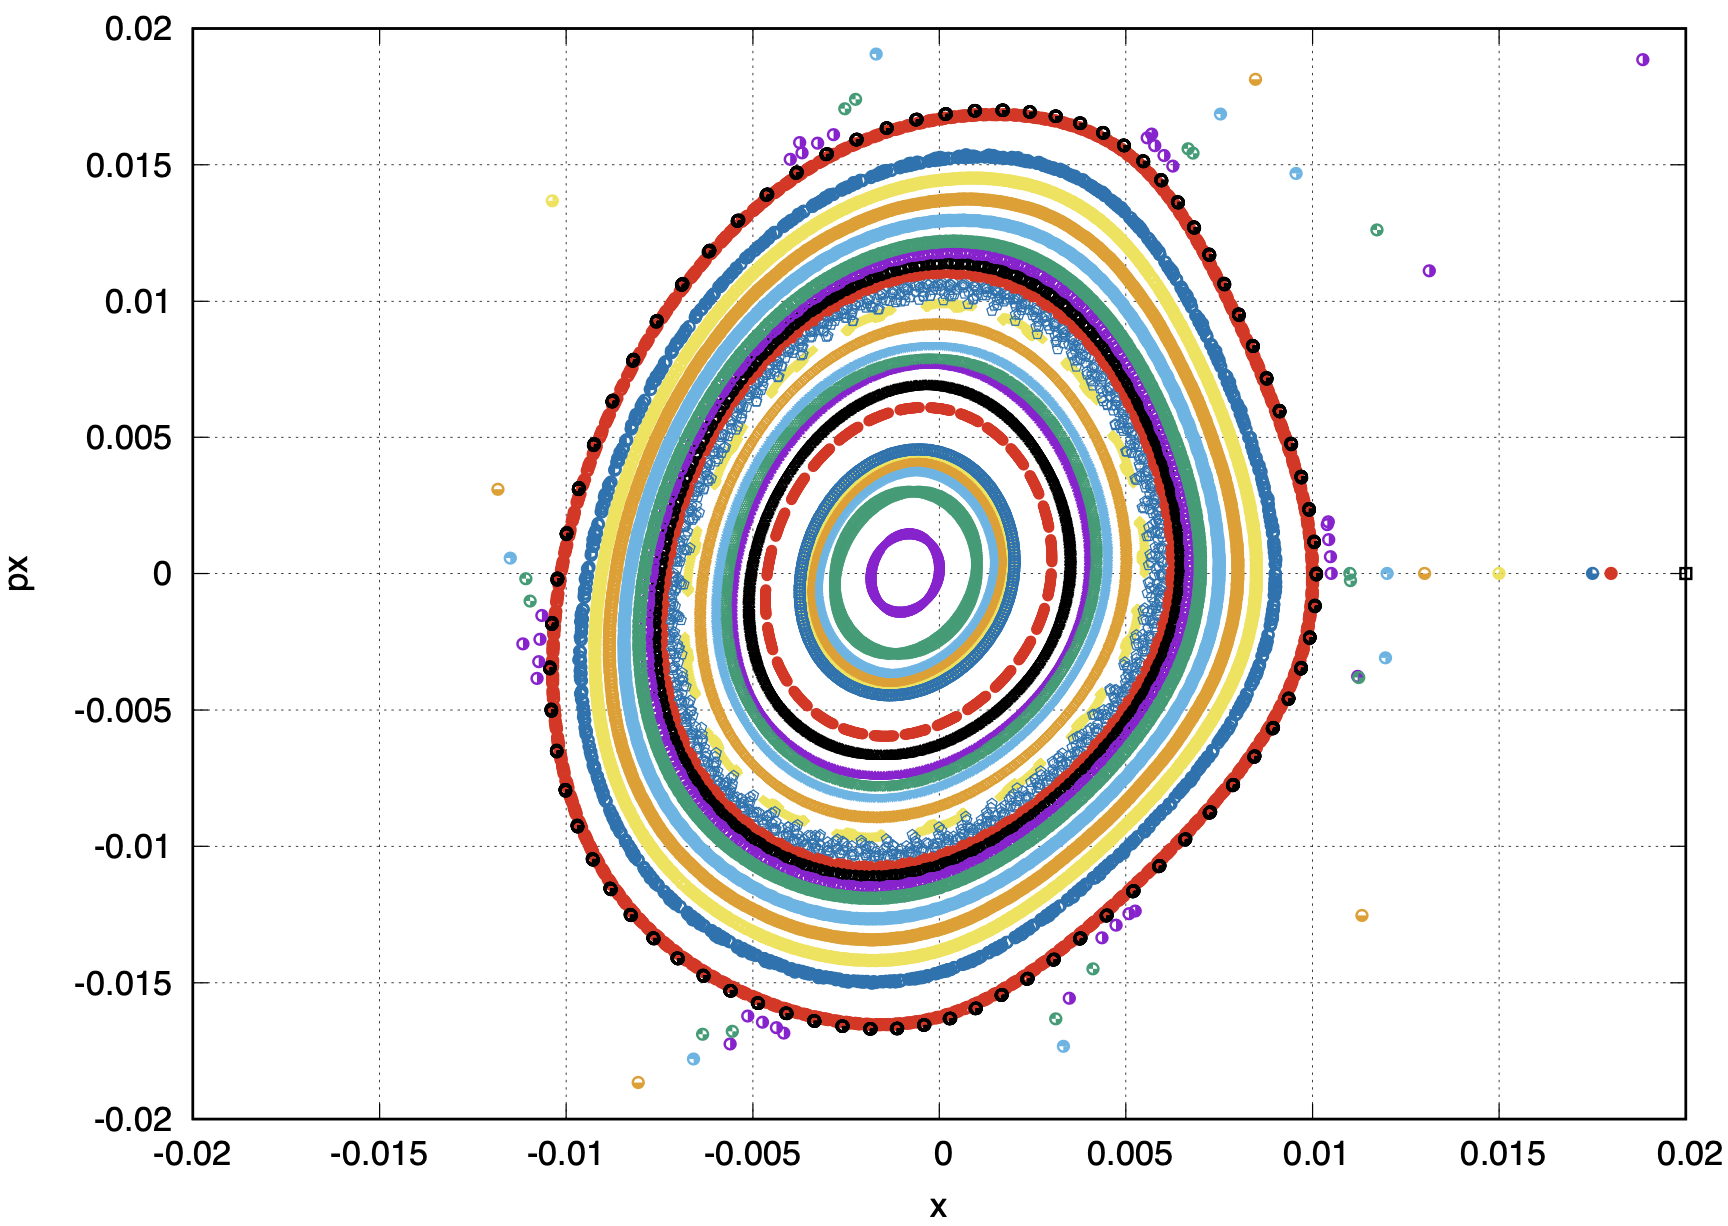
\includegraphics[width=\linewidth]{img/dyn_aper_x_AS}};
			\end{tikzpicture}
		\end{minipage}
		\begin{minipage}{0.5\linewidth}
			\begin{tikzpicture}
			\node (cone) at (0,0) {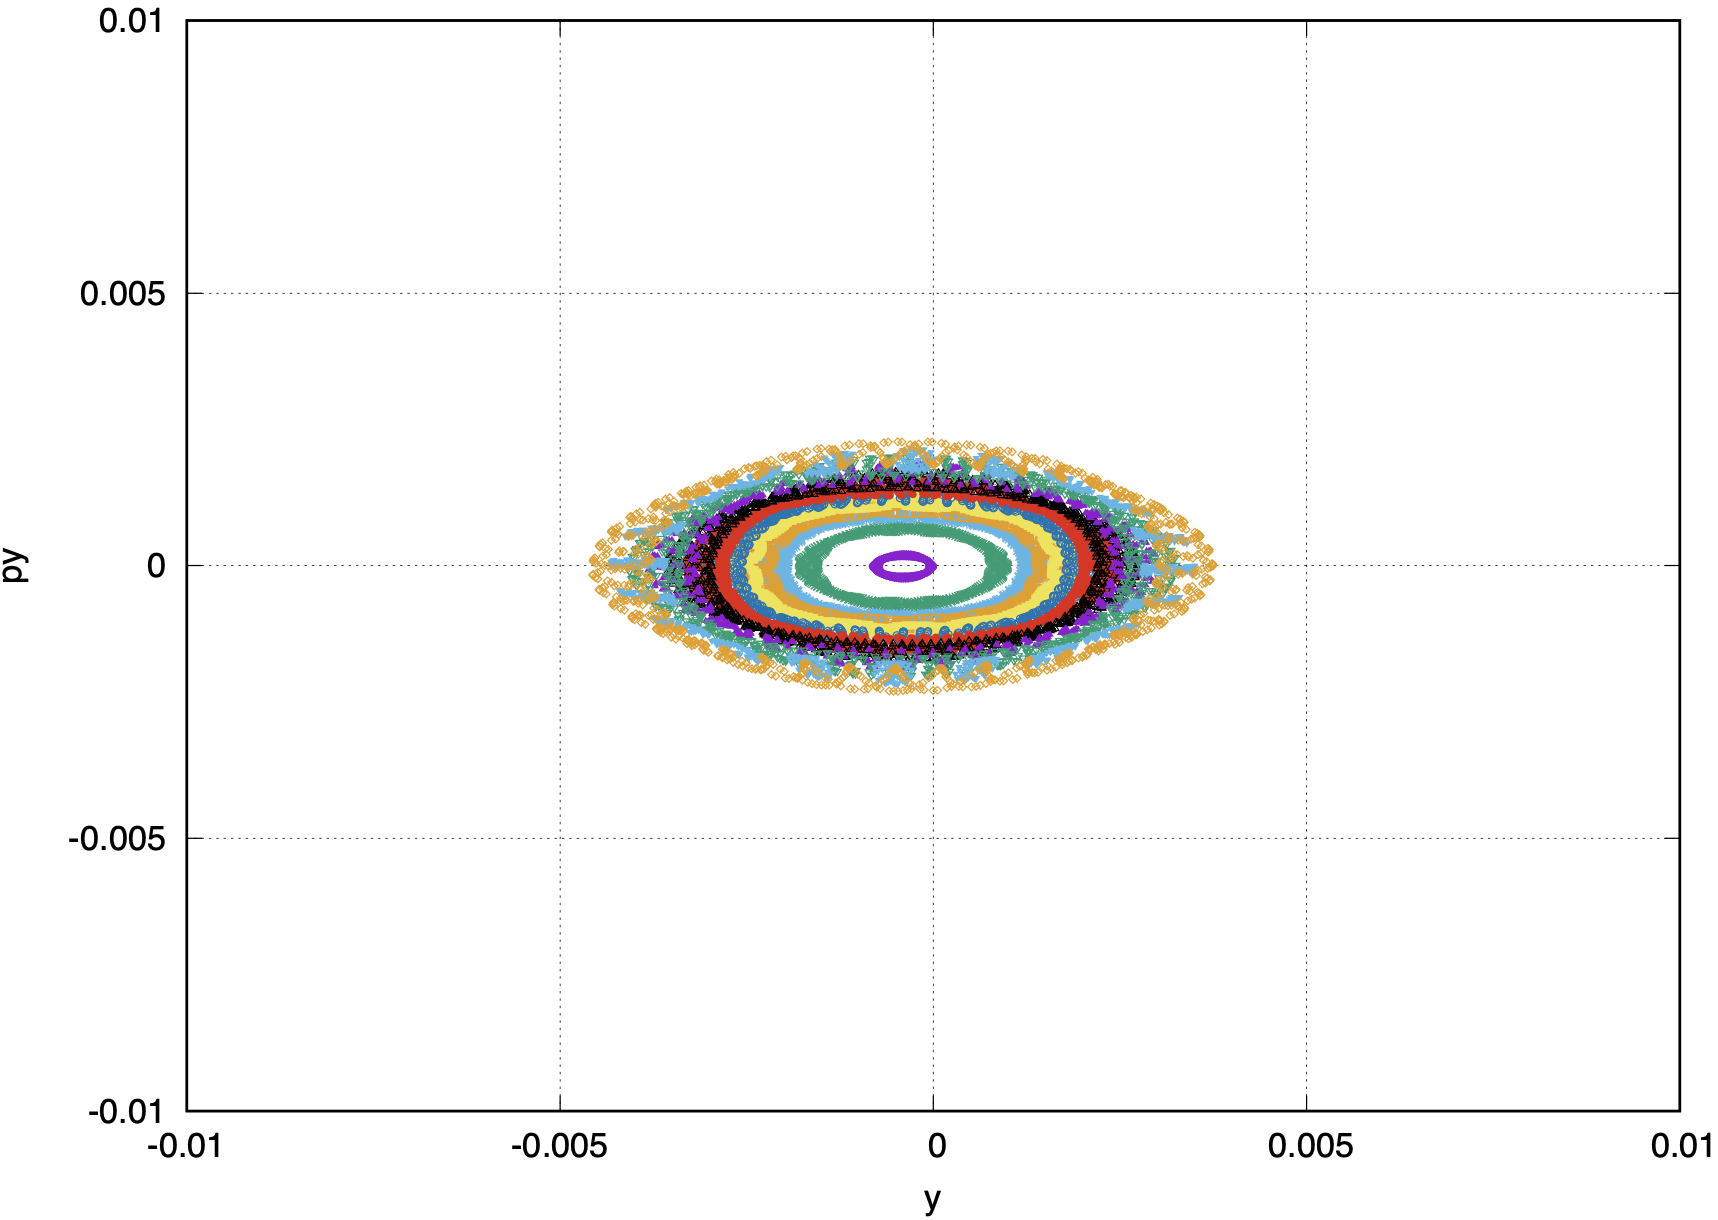
\includegraphics[width=\linewidth]{img/dyn_aper_y_AS}};
			\end{tikzpicture}
		\end{minipage}
		}
	\column{.33}
	\block{}{
	\begin{minipage}{0.5\linewidth}
			\begin{tikzpicture}
			\node (cone) at (0,0) {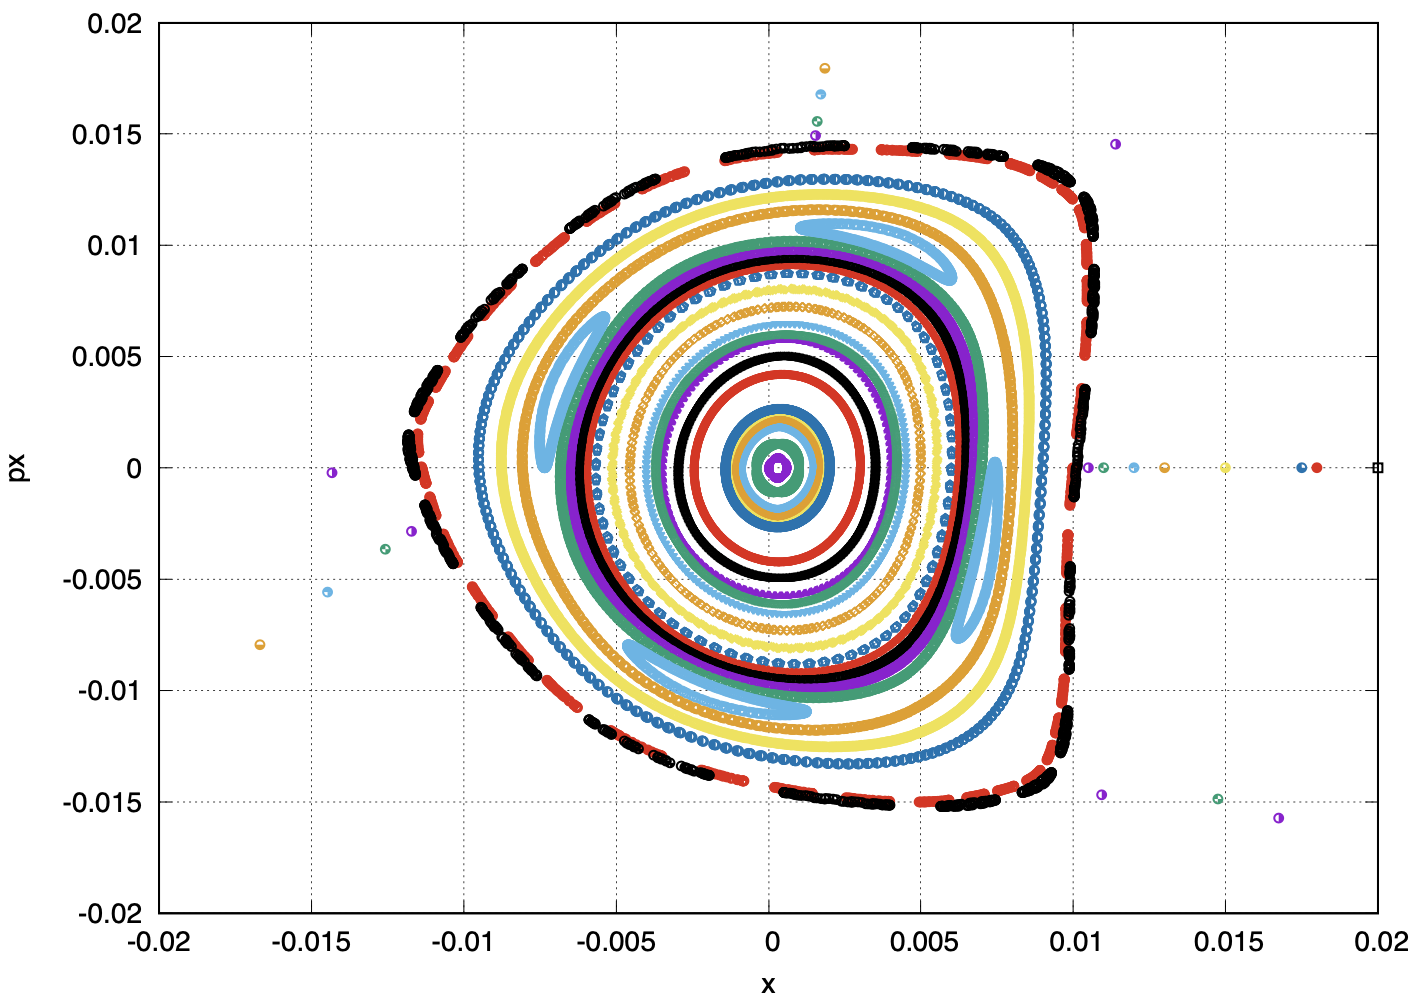
\includegraphics[width=\linewidth]{img/dyn_aper_x_ion}};
			\end{tikzpicture}
		\end{minipage}
		\begin{minipage}{0.5\linewidth}
			\begin{tikzpicture}
			\node (cone) at (0,0) {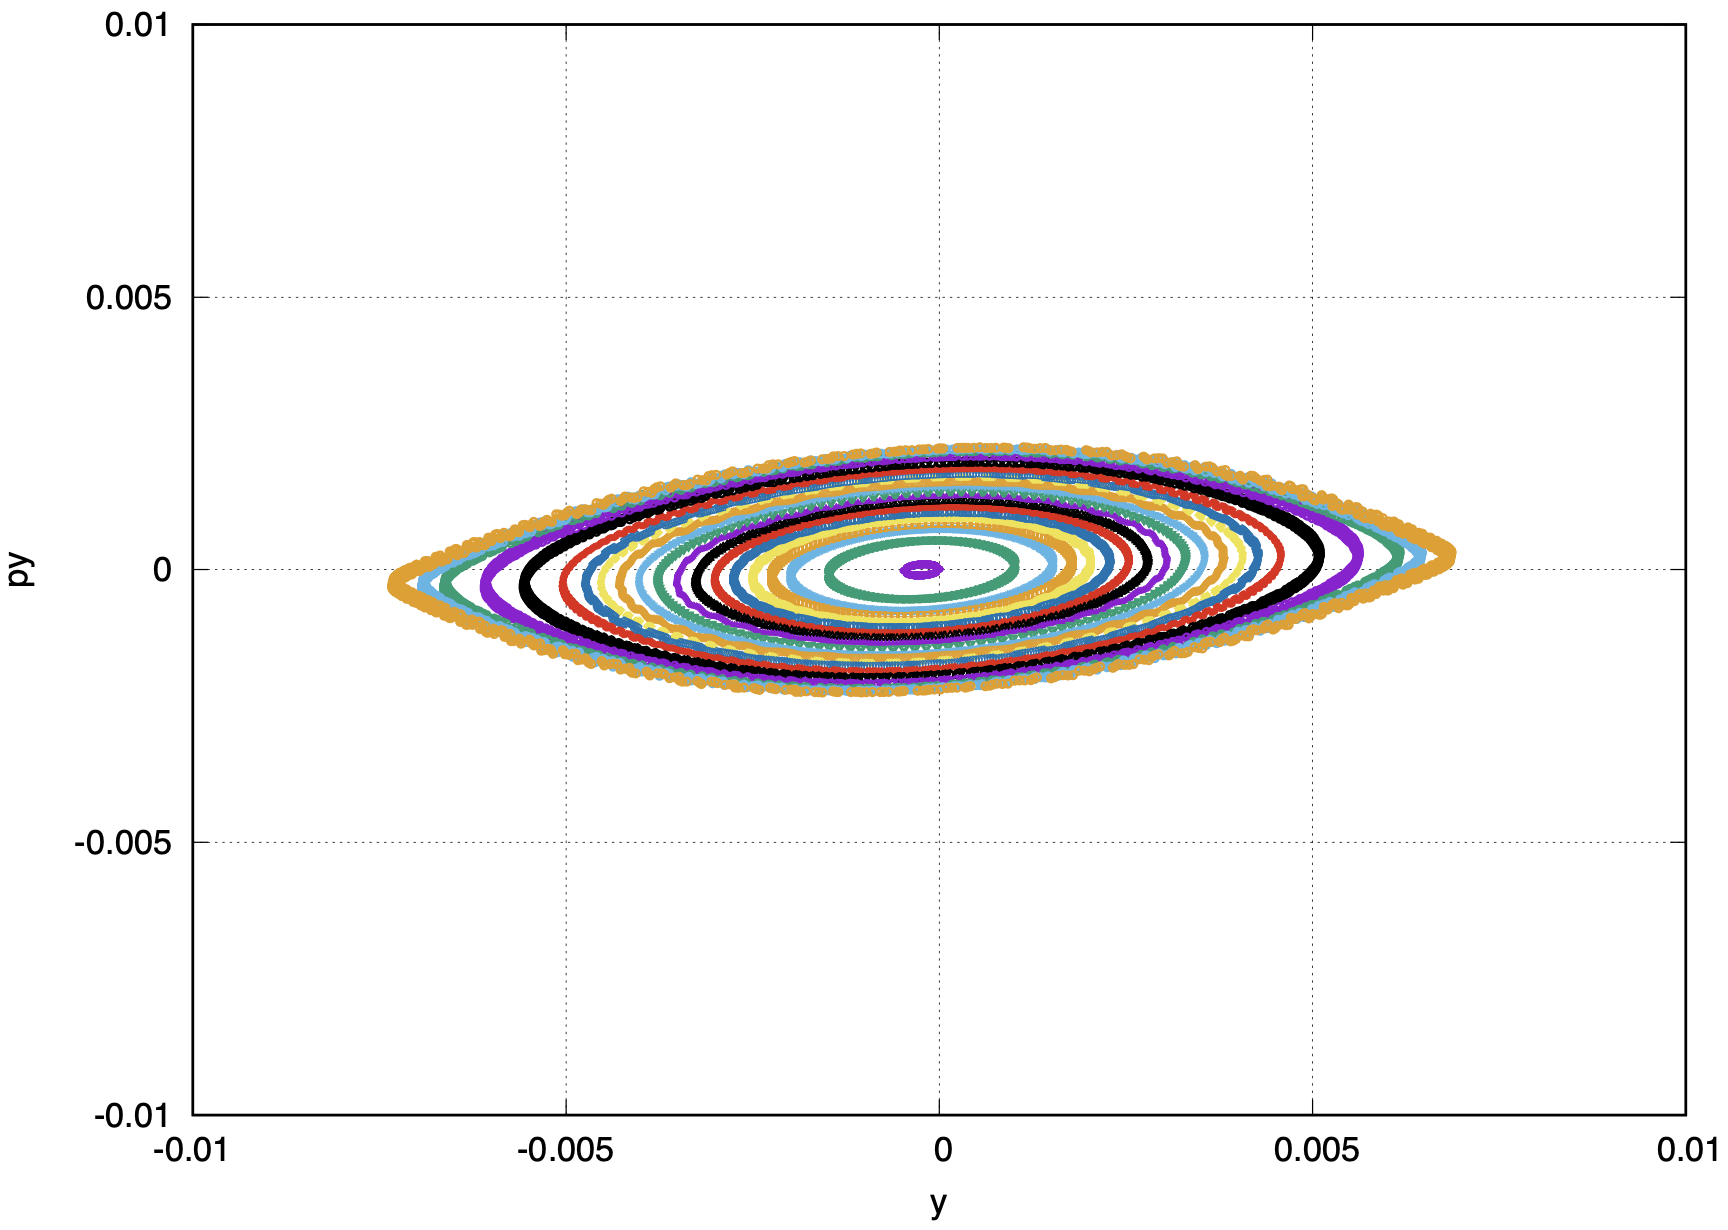
\includegraphics[width=\linewidth]{img/dyn_aper_y_ion}};
			\end{tikzpicture}
		\end{minipage}		
	}
\end{columns}

\begin{columns}
	\column{.5}
	\block{CONCLUSION}{
	\par	For proton mode of NICA collider applied method of superperiodic modulation to increase transition energy (change $\gamma_{tr}$ from $7,1$ to $15$). In this case two options of dispersion suppression on the edges of arc can be considered: suppression with edge superperiods and suppression with only two families of quadrupoles. Each option has it is own features, but both of them can be used on NICA collider.
	}
	\column{.5}
	\block{REFERENCES}{
	 
	\par [1] Yu. V. Senichev and A. N. Chechenin. Theory of “Resonant” Lattices for Synchrotrons with Negative Momentum Compaction Factor. Journal of Experimental and Theoretical Physics, 2007, Vol. 105, No. 5, pp. 988–997.
	\par [2] Yu. V. Senichev and A. N. Chechenin. Construction of “Resonant” Magneto-Optical Lattices with Controlled Momentum Compaction Factor Journal of Experimental and Theoretical Physics, 2007, Vol. 105, No. 6, pp. 1141–1156.
	}

\end{columns}

\end{document}